\documentclass[a4paper,twoside]{article}
% My LaTeX preamble file - by Nathaniel Dene Hoffman
% Credit for much of this goes to Olivier Pieters (https://olivierpieters.be/tags/latex)
% and Gilles Castel (https://castel.dev)
% There are still some things to be done:
% 1. Update math commands using mathtools package (remove ddfrac command and just override)
% 2. Maybe abbreviate \imath somehow?
% 3. Possibly format for margin notes and set new margin sizes
% First, some encoding packages and useful formatting
%--------------------------------------------------------------------------------------------
\usepackage{import}
\usepackage{pdfpages}
\usepackage{transparent}
\usepackage[l2tabu,orthodox]{nag}   % force newer (and safer) LaTeX commands
\usepackage[utf8]{inputenc}         % set character set to support some UTF-8
                                    %   (unicode). Do NOT use this with
                                    %   XeTeX/LuaTeX!
\usepackage[T1]{fontenc}
\usepackage[english]{babel}         % multi-language support
\usepackage{sectsty}                % allow redefinition of section command formatting
\usepackage{tabularx}               % more table options
\usepackage{booktabs}
\usepackage{titling}                % allow redefinition of title formatting
\usepackage{imakeidx}               % create and index of words
\usepackage{xcolor}                 % more colour options
\usepackage{enumitem}               % more list formatting options
\usepackage{tocloft}                % redefine table of contents, new list like objects
\usepackage{subfiles}               % allow for multifile documents

% Next, let's deal with the whitespaces and margins
%--------------------------------------------------------------------------------------------
\usepackage[centering,margin=1in]{geometry}
\setlength{\parindent}{0cm}
\setlength{\parskip}{2ex plus 0.5ex minus 0.2ex} % whitespace between paragraphs

% Redefine \maketitle command with nicer formatting
%--------------------------------------------------------------------------------------------
\pretitle{
  \begin{flushright}         % align text to right
    \fontsize{40}{60}        % set font size and whitespace
    \usefont{OT1}{phv}{b}{n} % change the font to bold (b), normally shaped (n)
                             %   Helvetica (phv)
    \selectfont              % force LaTeX to search for metric in its mapping
                             %   corresponding to the above font size definition
}
\posttitle{
  \par                       % end paragraph
  \end{flushright}           % end right align
  \vskip 0.5em               % add vertical spacing of 0.5em
}
\preauthor{
  \begin{flushright}
    \large                   % font size
    \lineskip 0.5em          % inter line spacing
    \usefont{OT1}{phv}{m}{n}
}
\postauthor{
  \par
  \end{flushright}
}
\predate{
  \begin{flushright}
  \large
  \lineskip 0.5em
  \usefont{OT1}{phv}{m}{n}
}
\postdate{
  \par
  \end{flushright}
}

% Mathematics Packages
\usepackage[Gray,squaren,thinqspace,cdot]{SIunits}      % elegant units
\usepackage{amsmath}                                    % extensive math options
\usepackage{amsfonts}                                   % special math fonts
\usepackage{mathtools}                                  % useful formatting commands
\usepackage{amsthm}                                     % useful commands for building theorem environments
\usepackage{amssymb}                                    % lots of special math symbols
\usepackage{mathrsfs}                                   % fancy scripts letters
\usepackage{cancel}                                     % cancel lines in math
\usepackage{esint}                                      % fancy integral symbols
\usepackage{relsize}                                    % make math things bigger or smaller
%\usepackage{bm}                                         % bold math!
\usepackage{slashed}

\newcommand\ddfrac[2]{\frac{\displaystyle #1}{\displaystyle #2}}    % elegant fraction formatting
\allowdisplaybreaks[1]                                              % allow align environments to break on pages

% Ensure numbering is section-specific
%--------------------------------------------------------------------------------------------
\numberwithin{equation}{section}
\numberwithin{figure}{section}
\numberwithin{table}{section}

% Citations, references, and annotations
%--------------------------------------------------------------------------------------------
\usepackage[small,bf,hang]{caption}        % captions
\usepackage{subcaption}                    % adds subfigure & subcaption
\usepackage{sidecap}                       % adds side captions
\usepackage{hyperref}                      % add hyperlinks to references
\usepackage[noabbrev,nameinlink]{cleveref} % better references than default \ref
\usepackage{autonum}                       % only number referenced equations
\usepackage{url}                           % urls
\usepackage{cite}                          % well formed numeric citations
% format hyperlinks
\colorlet{linkcolour}{black}
\colorlet{urlcolour}{blue}
\hypersetup{colorlinks=true,
            linkcolor=linkcolour,
            citecolor=linkcolour,
            urlcolor=urlcolour}

% Plotting and Figures
%--------------------------------------------------------------------------------------------
\usepackage{tikz}          % advanced vector graphics
\usepackage{pgfplots}      % data plotting
\usepackage{pgfplotstable} % table plotting
\usepackage{placeins}      % display floats in correct sections
\usepackage{graphicx}      % include external graphics
\usepackage{longtable}     % process long tables

% use most recent version of pgfplots
\pgfplotsset{compat=newest}

% Misc.
%--------------------------------------------------------------------------------------------
\usepackage{todonotes}  % add to do notes
\usepackage{epstopdf}   % process eps-images
\usepackage{float}      % floats
\usepackage{stmaryrd}   % some more nice symbols
\usepackage{emptypage}  % suppress page numbers on empty pages
\usepackage{multicol}   % use this for creating pages with multiple columns
\usepackage{etoolbox}   % adds tags for environment endings
\usepackage{tcolorbox}  % pretty colored boxes!


% Custom Commands
%--------------------------------------------------------------------------------------------
\newcommand\hr{\noindent\rule[0.5ex]{\linewidth}{0.5pt}}                % horizontal line
\newcommand\N{\ensuremath{\mathbb{N}}}                                  % blackboard set characters
\newcommand\R{\ensuremath{\mathbb{R}}}
\newcommand\Z{\ensuremath{\mathbb{Z}}}
\newcommand\Q{\ensuremath{\mathbb{Q}}}
%\newcommand\C{\ensuremath{\mathbb{C}}}
\renewcommand{\arraystretch}{1.2}                                       % More space between table rows (could be 1.3)
\newcommand{\Cov}{\mathrm{Cov}}
\newcommand\D{\mathrm{D}}
\newcommand*{\dbar}{\ensuremath{\text{\dj}}}

\newcommand{\incfig}[2][1]{%
    \def\svgwidth{#1\columnwidth}
    \import{./figures/}{#2.pdf_tex}
}

% Custom Environments
%--------------------------------------------------------------------------------------------
\newcommand{\lecture}[3]{\hr\\{\centering{\large\textsc{Lecture #1: #3}}\\#2\\}\hr\markboth{Lecture #1: #3}{\rightmark}}   % command to title lectures
\usepackage{mdframed}
\theoremstyle{plain}
\newmdtheoremenv[nobreak]{theorem}{Theorem}[section]
\newtheorem{corollary}{Corollary}[theorem]
\newtheorem{lemma}[theorem]{Lemma}
\theoremstyle{definition}
\newtheorem*{ex}{Example}
\newmdtheoremenv[nobreak]{definition}{Definition}[section]
\theoremstyle{remark}
\newtheorem*{remark}{Remark}
\newtheorem*{claim}{Claim}
\AtEndEnvironment{ex}{\null\hfill$\diamond$}%
% Note: A proof environment is already provided in the amsthm package
\tcbuselibrary{breakable}
\newenvironment{note}[1]{\begin{tcolorbox}[
    arc=0mm,
    colback=white,
    colframe=white!60!black,
    title=#1,
    fonttitle=\sffamily,
    breakable
]}{\end{tcolorbox}}
\newenvironment{problem}{\begin{tcolorbox}[
    arc=0mm,
    breakable,
    colback=white,
    colframe=black
]}{\end{tcolorbox}}

% Header and Footer
%--------------------------------------------------------------------------------------------
% set header and footer
\usepackage{fancyhdr}                       % header and footer
\pagestyle{fancy}                           % use package
\fancyhf{}
\fancyhead[LE,RO]{\textsl{\rightmark}}      % E for even (left pages), O for odd (right pages)
\fancyfoot[LE,RO]{\thepage}
\fancyfoot[LO,RE]{\textsl{\leftmark}}
\setlength{\headheight}{15pt}


% Physics
%--------------------------------------------------------------------------------------------
\usepackage[arrowdel]{physics}      % all the usual useful physics commands
\usepackage{feyn}                   % for drawing Feynman diagrams
%\usepackage{bohr}                   % for drawing Bohr diagrams
%\usepackage{tikz-feynman}
\usepackage{elements}               % for quickly referencing information of various elements
\usepackage{tensor}                 % for writing tensors and chemical symbols

% Finishing touches
%--------------------------------------------------------------------------------------------
\author{Nathaniel D. Hoffman}

\title{33-765 Homework 8}
\date{\today}
\begin{document}
\maketitle

\section*{29. Joule-Thomson Coefficient for the van der Waals Gas}
Let's combine two subjects of inquiry: We know from class what the Joule-Thomson effect is, and we know that it is boring for the ideal gas. But now we have an equation of state for a more realistic gas!\ What does this say about the Joule-Thomson coefficient? We start by writing the van der Waals equation in rescaled variables:
\begin{equation}
    V_c = 3Nb \qquad k_B T_c = \frac{8a}{27b} \qquad P_c = \frac{a}{27b^2}
\end{equation}
and hence define
\begin{equation}
    \tilde{T} = \frac{T}{T_c} \qquad \tilde{P} = \frac{P}{P_c} \qquad \tilde{V} = \frac{V}{V_c}
\end{equation}

\begin{itemize}
    \item[1.] Show that in the reduced variables $ \tilde{T} $, $ \tilde{V} $, and $ \tilde{N} $, the thermal equation of state reads $ (\tilde{P}+ 3 \tilde{V}^{-2})(3\tilde{V}-1)=8\tilde{T} $.
        \begin{problem}
            The thermal equation of state for a van der Waals gas is
            \begin{equation}
                P = \frac{N k_B T}{V - bN} - \frac{a N^2}{V^2}
            \end{equation}
            We can write our scaled variables in terms of the regular ones
            \begin{equation}
                \tilde{T}= \frac{27b k_B T}{8a} \qquad \tilde{P}= \frac{27b^2 P}{a} \qquad \tilde{V}= \frac{V}{3bN}
            \end{equation}
            and substitute those into our equation of state:
            \begin{align}
                \frac{a}{27b^2} \tilde{P}&= \frac{N \tilde{T}\left( \frac{8a}{27b} \right)}{bN(3 \tilde{V} - 1)} - \frac{aN^2}{9 b^2 \tilde{V}^2 N^2} \\
                &= \frac{8a \tilde{T}}{27b^2 (3 \tilde{V}- 1)} - \frac{a}{9 b^2\tilde{V}^2} \\
                \tilde{P} &= \frac{8\tilde{T}}{(3\tilde{V}-1)} - \frac{3}{\tilde{V}^2} \\
                \frac{8\tilde{T}}{(3\tilde{V}-1)} &= (\tilde{P}+3\tilde{V}^{-2}) \\
                8\tilde{T} &= (\tilde{P}+ 3\tilde{V}^{-2})(3\tilde{V}-1)
            \end{align}
        \end{problem}
    \item[2.] Find the relationship between $ \tilde{P} $ and $ \tilde{V} $ (with $ \tilde{T} $ eliminated!) that holds when the Joule-Thomson coefficient $ \mu_{\text{JT}} = 0 $. Note, it turns out that for pressures below this so-called ``inversion curve'' $ \tilde{P}_{\text{inv}}(\tilde{V}) $, we have $ \mu_{\text{JT}} > 0 $.
        \begin{problem}
            The Joule-Thomsom coefficient equation states that
            \begin{equation}
                \mu_{\text{JT}} = - \frac{\tilde{V}}{Nc_P} (\tilde{T} \alpha - 1) = 0 \implies \tilde{T} = \frac{1}{\alpha} = \tilde{V} \eval{\pdv{\tilde{T}}{\tilde{V}}}_{P,N}
            \end{equation}
            We can take this derivative from the equation of state:
            \begin{equation}
                \tilde{T}= \tilde{V}\left( \frac{3(2-3\tilde{V}+\tilde{P}\tilde{V}^3)}{\tilde{V}^3} \right)
            \end{equation}
            Substituting this back into the original equation and solving for $ \tilde{P} $, we find that
            \begin{equation}
                \tilde{P}_{\text{inv}}(\tilde{V}) = \frac{9}{\tilde{V}^2} (2 \tilde{V}-1)
            \end{equation}
        \end{problem}
    \item[3.] Using the scaled thermal equations of state, show that the volume on the inversion curve satisfies $ \tilde{V}^{-1} = 3 - \sqrt{4\tilde{T}/3} $.
        \begin{problem}
            To do this, we just substitute the new equation we found into the original:
            \begin{align}
                \left( \frac{9}{\tilde{V}^2} (2\tilde{V} - 1) + \frac{3}{\tilde{V}^2} \right)(3\tilde{V} - 1) &= 8\tilde{T} \\
                \frac{6(1-3\tilde{V})^2}{\tilde{V}^2} &= 8\tilde{T} \\
                \frac{(1-3\tilde{V})^2}{\tilde{V}^2} &= \frac{4}{3} \tilde{T} \\
                \frac{1-3\tilde{V}}{\tilde{V}} &= - \sqrt{\frac{4}{3} \tilde{T}} \\
                \frac{1}{\tilde{V}} - 3 &= - \sqrt{\frac{4}{3} \tilde{T}} \\
                \frac{1}{\tilde{V}} &= 3 - \sqrt{4\tilde{T}/3}
            \end{align}
            Here I chose the negative root because it gave me the answer I wanted, clever right?
        \end{problem}
    \item[4.] Inserting this into $ \tilde{P}_{\text{inv}} $, you get the inversion curve in the $\tilde{T}-\tilde{P}$ diagram. Plot it!\ The part under the curve is the region that has a positive Joule-Thomson coefficient and will thus cool when subjected to the Joule-Thomson process.
        \begin{problem}
            \begin{align}
                \tilde{P}(\tilde{T}) &= \frac{9}{\left( 3- \sqrt{4\tilde{T}/3} \right)^2} \left( \frac{2}{3- \sqrt{4\tilde{T}/3}} - 1 \right) \\
                &= \left( \frac{6}{\sqrt{12\tilde{T} - 9}} - 1 \right)\left( \sqrt{12\tilde{T}} - 9 \right)^2 \\
                &= 24 \sqrt{3\tilde{T}} - 12 \tilde{T} - 27
            \end{align}
            See \Cref{fig:problem_29_4} for the plot (I couldn't figure out how to put tildes in in Mathematica, sorry, just pretend they're there).
        \end{problem}
        \begin{figure}[h]
            \centering
            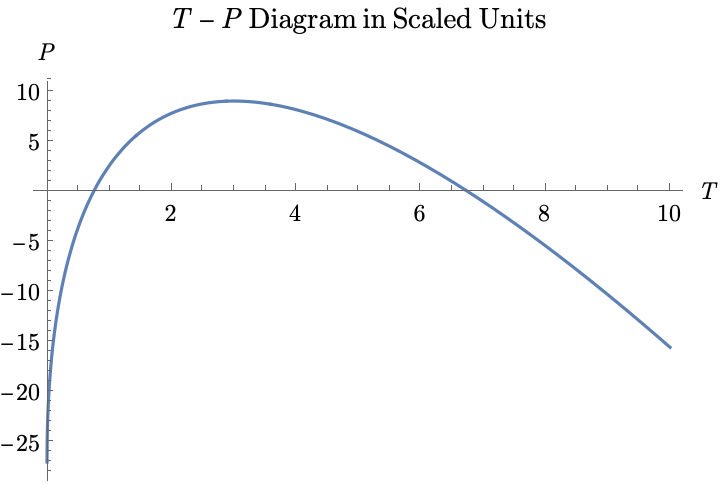
\includegraphics[width=\textwidth]{Problem_29_5_Plot.png}
            \caption{Plot for Problem 29.4}
            \label{fig:problem_29_4}
        \end{figure}
    \item[5.] For hydrogen ($ \text{H}_2 $) we have $ T_c = -240\degreecelsius $ and $ P_c = 12.7\text{atm} $, while for carbon dioxide ($ \text{CO}_2 $) we have $ T_c = 31.2\degreecelsius $ and $ P_c = 72.8\text{atm} $. Do these gases heat up or cool down under a throttled expansion at room temperature and pressure?
        \begin{problem}
            Room temperature and pressure are about $ 22\degreecelsius $ and $ 1\text{atm} $. I'll convert everything to Kelvin so that we don't run into problems with negative temperature. This means room temperature is $ 295\kelvin $ and the critical temperatures for hydrogen and carbon dioxide are $ 33\kelvin $ and $ 304.2\kelvin $ respectively. This gives us
            \begin{equation}
                \tilde{P} = \frac{P}{P_c} = \frac{1}{12.7} = 0.078 \qquad \tilde{T}= \frac{295}{33} = 8.94
            \end{equation}
            for Hydrogen and
            \begin{equation}
                \tilde{P} = \frac{1}{72.8} = 0.0137 \qquad \tilde{T} = \frac{295}{304.2} = 0.97
            \end{equation}
            for carbon dioxide.


            Examining the plot from the previous question, we can see that the point for Hydrogen gas falls above the curve while the point for carbon dioxide falls below it, so carbon dioxide will cool under the Joule-Thomson process while Hydrogen gas will not.
        \end{problem}
\end{itemize}


\section*{30. Ice Skating}
First, a few facts: (1) Icebergs contain freshwater, and only about $ 10\% $ of an iceberg is visible above the ocean's surface. (2) The density of sea water is about $ 1.025\gram/\centi\meter^3 $. (3) It takes about $ 334\kilo\joule $ to melt one kilogram of ice (from just below freezing to just above freezing). Now here comes the problem you will be able to solve using these data:
\begin{itemize}
    \item[1.] What is the slope of the melting curve in the T-P diagram of water at atmospheric pressure?
        \begin{problem}
            First, we know from the Clausius-Clapeyron equation that
            \begin{equation}
                \dv{P}{T} = \frac{L}{T \Delta V}
            \end{equation}
            $ L $ is the latent heat of the transition, given in the problem as $ 334\kilo\joule $. $ T $ is the temperature at which ice freezes/melts, which is $ \sim 273\kelvin $. Finally, we can use the first and second facts to determine the density of ice to be $ 0.9 \times 1025\kilo\gram/\meter^3 = 922.5\kilo\gram/\meter^3 $. The density of water is defined as $ 1000\kilo\gram/\meter^3 $, and we want to find the change in volume per particle, since that's what $ L $ is written in terms of. Therefore, we don't care about the mass: $ \Delta V = \frac{1}{922.5\meter^3} - \frac{1}{1000\meter^3} = -8.4 \times 10^{-5} \meter^3 $. Plugging this all in, we find that
            \begin{equation}
                \dv{P}{T} = \frac{334000\joule/\kilo\gram}{273\kelvin(-8.4 \times 10^{-5} \meter^3)} = -1.45 \times 10^7 \pascal/\kelvin
            \end{equation}
        \end{problem}
    \item[2.] Most ice rinks operate at about $ -7\degreecelsius $. How heavy would a person have to be so that the pressure exerted on the ice through the blades of that person's skates will pressure-melt the ice? (Estimate the area of an ice skate's blade.)
        \begin{problem}
            If we take our result from the previous section, we can recognize the units to be $ \pascal/\kelvin = \left( \frac{\newton}{\meter^2} \right)\kelvin $, so we need to multiply our result by $ \Delta T = - 7\kelvin $ to get force and area:
            \begin{equation}
                -1.45 \times 10^7 \pascal/\kelvin * -7\kelvin = 1.015 \times 10^8 \newton/\meter^2
            \end{equation}
            I'll make a guess that the average pair of ice skates have an area of $ 0.0004\meter^2 $, so it will take
            \begin{equation}
                1.015 \times 10^8 \newton/\meter^2 * 0.0004\meter^2 = 4.06\times 10^4 N
            \end{equation}
            to melt it. Approximating $ g = 10\meter/\second^2 $, we find that the required mass is
            \begin{equation}
                4060\kilo\gram = 8950.768\text{lbs}
            \end{equation}
            I doubt this is true, since the melting is what makes the ice skate move easily across the surface, but I don't know where I went wrong here. The average person should be able to melt the ice.
        \end{problem}
\end{itemize}

\section*{31. Equipartition Theorem}
Consider a Hamiltonian $ H(\{p,q\}) $ on phase space. Let $ x_i $ be any of the $ 6N $ coordinates, for instance, it could be $ p_{27,y} $ or $ q_{1673536,x} $. Let $ \ev{\cdot} $ denote the canonical average (i.e., the average over the canonical state $ P_{\text{can}}(\{p,q\}) $).
\begin{itemize}
    \item[1.] Prove that the following is true: $ \ev{x_i \pdv{H}{x_j}} = k_B T \delta_{ij} $. (Hint: Parameter differentiation and integration by parts)
        \begin{problem}
            \begin{align}
                \ev{x_i \pdv{H}{x_j}} &= \int \dd{\Gamma} x_i \pdv{H}{x_j} P_{\text{can}}(\Gamma) \\
                &= \int  x_i \dd{\left( - \frac{1}{\beta} P_{\text{can}}(\Gamma) \right)} \\
                &= \eval{x_i \left( - \frac{1}{\beta} P_{\text{can}}(\Gamma) \right)}_{\partial\Gamma} + \int \dd{\Gamma} \frac{1}{\beta} P_{\text{can}}(\Gamma) \pdv{x_i}{x_j}
            \end{align}
            Since the variables don't depend on each other, $ \pdv{x_i}{x_j} $ will give us a $ \delta $-function. The first term is zero because the probability distribution must vanish at the boundary.
            \begin{equation}
                \ev{x_i \pdv{H}{x_j}} = \frac{1}{\beta} \int P_{\text{can}}(\Gamma) \delta_{ij} \dd{\Gamma} = k_B T \delta_{ij}
            \end{equation}
            since $ \int P_{\text{can}}(\Gamma) \dd{\Gamma} = 1 $ by normalization.
        \end{problem}
    \item[2.] If the Hamiltonian contains a term $ A x^n $ and this is the only occurrence of $ x $, prove that $ \ev{A x^n} = \frac{1}{n} k_B T $.
        \begin{problem}
            We can rewrite
            \begin{equation}
                \ev{Ax^n} = \ev{\left( \frac{1}{n} x \right)\left( Anx^{n-1} \right)} = \frac{1}{n} \ev{x Anx^{n-1}}
            \end{equation}
            Noticing that $ \pdv{H}{x} = Anx^{n-1} $, we use part 1 to write:
            \begin{equation}
                \ev{A x^n} = \frac{1}{n} \ev{x \pdv{H}{x}} = \frac{k_BT}{n} 
            \end{equation}
        \end{problem}
    \item[3.] For the ``standard'' kinetic energy and $ p_i $, one of the (scalar) momentum coordinates, prove that $ \ev{\frac{p_i^2}{2m}} = \frac{1}{2} k_B T $.
        \begin{problem}
            The ``standard'' kinetic energy term makes the Hamiltonian have the form $ H = \frac{p^2}{2m} + \Phi(\{q\}) $, so this problem has the same form as the previous problem with $ n = 2 $.
        \end{problem}
\end{itemize}

\section*{32. Hypervirial and Temperature}
Let $ \vb{\Gamma} = \{\vb{p}_1,\cdots, \vb{p}_N, \vb{q}_1, \cdots, \vb{q}_N\} $ denote a point in $ 6N $-dimensional phase space, and let $ \vb{B}(\vb{\Gamma}) $ be a vector field in phase space. Let us furthermore denote the gradient operator in phase space by $ \grad_{\vb{\Gamma}} = \left( \pdv{p_{1x}}, \pdv{p_{1y}}, \pdv{p_{1z}}, \pdv{p_{2z}}, \cdots, \pdv{q_{Nz}} \right) $.
\begin{itemize}
    \item[1.] Use Gauss' theorem to argue that $ \int \dd{\vb{\Gamma}} \grad_{\vb{\Gamma}} \vdot \{\vb{B}(\vb{\Gamma}) e^{- \beta H(\vb{\Gamma})}\} = 0 $.
        \begin{problem}
            I don't understand how this follows. Converting to the surface integral we get a unit vector pointing outward from the surface, but I don't really know what to do with that.
        \end{problem}
    \item[2.] Prove the amazing fact that every choice of $ \vb{B} $ leads to an expression for the temperature: $ k_B T = \ev{\vb{B} \vdot \grad_{\vb{\Gamma}} H} / \ev{\grad_{\vb{\Gamma}} \vdot \vb{B}} $.
        \begin{problem}
            \begin{align}
                \ev{\vb{B}(\vb{\Gamma} \vdot \grad_{\vb{\Gamma}}H)} &= \int \dd{\vb{\Gamma}} \vb{B}(\vb{\Gamma}) \vdot \left( \grad_{\vb{\Gamma}} P_{\text{can}}(\vb{\Gamma}) \right)\\
                &= \int \dd{\vb{\Gamma}} \vb{B}(\vb{\Gamma}) \vdot \grad_{\vb{\Gamma}} \left( - \frac{1}{\beta} P_{\text{can}}(\vb{\Gamma}) \right) \\
                &= \eval{\vb{B}(\vb{\Gamma}) \vdot \grad_{\vb{\Gamma}} \left( H(\vb{\Gamma}) P_{\text{can}}(\vb{\Gamma}) \right)}_{\partial\Gamma} + \int \frac{1}{\beta} \grad_{\vb{\Gamma}} \vdot \vb{B}(\vb{\Gamma}) P_{\text{can}}(\vb{\Gamma}) \dd{\vb{\Gamma}} \\ &+ \int \frac{1}{\beta} \grad_{\vb{\Gamma}} \vdot \left( \vb{B}(\vb{\Gamma}) P_{\text{can}}(\vb{\Gamma}) \right) \dd{\vb{\Gamma}} 
            \end{align}
            The first term is zero because the probability density vanishes on the boundary. The second term is zero because of what we know from question 32.1. Finally
            \begin{align}
                \ev{\vb{B}(\vb{\Gamma}) \vdot \grad_{\vb{\Gamma}} H} &= \frac{1}{\beta} \int \grad_{\vb{\Gamma}} \vdot \vb{B}(\vb{\Gamma}) P_{\text{can}}(\vb{\Gamma}) \dd{\vb{\Gamma}} \\
                &= \frac{1}{\beta} \ev{\grad_{\vb{\Gamma}} \vb{B}(\vb{\Gamma})} \\
                \implies k_B T = \ev{\vb{B} \vdot \grad_{\vb{\Gamma}} H} / \ev{\grad_{\vb{\Gamma}} \vdot \vb{B}}
            \end{align}
        \end{problem}
    \item[3.] For a standard Hamiltonian, $ H = K + \Phi = \sum_{i=1}^{N} \frac{\vb{p}_i^2}{2m} + \Phi(\vb{q}_1, \cdots, \vb{q}_N) $, calculate $ \grad_{\vb{\Gamma}} K $, $ \grad_{\vb{\Gamma}} \Phi $, and $ \grad_{\vb{\Gamma}} H $.
        \begin{problem}
            \begin{equation}
                \grad_{\vb{\Gamma}} K = \left\{\pdv{p_{1x}}\left[\left( \frac{(\sqrt{p_{1x}^2 + p_{1y}^2 + p_{1z}^2})^2}{2m} + \cdots\right] , \cdots, \underbrace{\pdv{q_{1x}} K}_{0}, \cdots \right)\right\} = \frac{1}{m} \left\{ p_{1x}, \cdots, 0, \cdots \right\}
            \end{equation}
            \begin{equation}
                \grad_{\vb{\Gamma}} \Phi = \left\{ \underbrace{\pdv{p_{1x}} \Phi}_{0}, \cdots, \pdv{q_{1x}} \Phi, \cdots \right\}
            \end{equation}
            \begin{equation}
                \grad_{\vb{\Gamma}} H = \grad_{\vb{\Gamma}} (K + \Phi) = \grad_{\vb{\Gamma}} K + \grad_{\vb{\Gamma}} \Phi = \left\{ \frac{p_{1x}}{m}, \cdots, \partial_{q_{1x}} \Phi, \cdots \right\}
            \end{equation}
        \end{problem}
    \item[4.] Choosing $ \vb{B}(\vb{\Gamma}) = \grad_{\vb{\Gamma}} K $, calculate the temperature implied by the new equation. This is called the ``kinetic temperature''.
        \begin{problem}
            \begin{align}
                k_B T &= \frac{\ev{\frac{1}{m^2} \sum_{p_{ni}} p_{ni}^2}}{\ev{\sum_{p_{ni}} \pdv{p_{ni}} \frac{p_{ni}}{m}}}\\
                &= \frac{\ev{\frac{1}{m^2} \sum_{p_{ni}} p_{ni}^2}}{\ev{\sum_{p_{ni}} \frac{1}{m}}}\\
                &= \frac{\ev{\frac{2}{m} \sum_{p_{ni}} \frac{p_{ni}^2}{2m}}}{\frac{3N}{m}}\\
                &= \frac{\frac{2}{m} \ev{K}}{\frac{3N}{m}}\\
                &= \frac{2}{3N} \ev{K} \\
                T &= \frac{2\ev{K}}{3N k_B} 
            \end{align}
        \end{problem}
    \item[5.] Repeat, but for the choice $ \vb{B}(\vb{\Gamma}) = \grad_{\vb{\Gamma}} \Phi $. This is called the ``configurational temperature''.
        \begin{problem}
            \begin{align}
                k_B T &= \frac{\ev{\sum_{q_{ni}} (\partial_{q_{ni}} \Phi)^2}}{\ev{\sum_{q_{ni}} \partial_{q_{ni}}^2 \Phi}}
            \end{align}
            I'm not sure how to simplify this at all.
        \end{problem}
\end{itemize}








\end{document}
